\documentclass[../../workflow.tex]{subfiles}
\graphicspath{{\subfix{../../img/}}}

\begin{document}

\section{T-Type Calcium Channel}
\etocignoretoctocdepth % of course, if we want to see something in local TOC...
\etocsettocstyle{\subsection*{\contentsname}}{}
\localtableofcontents


\newpage
\color{orange}

\textcolor{red}{Main results}:
\begin{itemize}
    \item Estimated number of activation gates for Drosophila T-Type ion channels is 3.
    \item Modeling the ion channel using Ohmic relationship between current and voltage
    did not procude good fits to observed current-voltage (I-V) relationship.
    \item The current-voltage relationship was reproduced when
    Goldman-Hodgkin-Katz (GHK) voltage flux equation was used instead of Ohmic current
    \item GHK equation models explicit relationship between current, voltage, temperature and
    intra-/extracellular ion concentrations.
    \item The fit of simulated I-V relatoinship to the observed data was improved when
    the steady-state activation function was shifted along $V$ axis,
    and corresponding time constant was scaled and shifted along $V$ axis (parameters for
    shifting and scaling were taken to be free parameters during optimization)
\end{itemize}

\color{black}

\subsection{Model}

T-Type Ca$^{2+}$ current was modelled using constant-field equation \parencite{huguenardSimulationCurrentsInvolved1992}:
\begin{equation}\label{eq_constant_field_equation}
    I_T(V) = m_T(V)^3 h_T(V) P z^2 \frac{VF^2}{RT}\frac{[Ca^{2+}]_{\text{inside}} - [Ca^{2+}]_{\text{outside}} \exp{[-zFV/(RT)]} }{1 - \exp{[-zFV/(RT)]}}
\end{equation}
where $m_T$ and $h_T$ correspond to the activation and inactivation gates,
P is the maximum permeability (scaled to either have the current amplitude observed
during the electrophysiological experiments reported in \parencite{jeongCaa1TFlyTtype2015}
(Section \ref{subsec_r5_simulations_t_type_current}), or to ), z is the valence of ion ($=2$ for Ca$^{2+}$),
$V$ is membrane potential in Volts, F is Faraday's constant ($\approx 9.6485 \times 10^{4} C\cdot \text{mol}^{-1}$),
$R$ is the universal gas constant
($\approx 8.3145 J/K^\circ \cdot \text{Mol}$), $T$ is temperature is Kelvin (here, $273.16+25=298.16^{\circ}$).
$[Ca^{2+}]_{\text{inside}}$ and $[Ca^{2+}]_{\text{outside}}$ are the concentrations of Ca$^{2+}$ inside and
outside the membrane. The values were set to $23 \times e^{-9}$ and $0.5 \times e^{-3}$ correspondingly,
from the motor neurons in Drosophila
\parencite{frankenhaeuserActionCalciumElectrical1957}.

Another approach to model the T-Type Ca$^{2+}$ current is by Ohm's law \parencite{huguenardSimulationCurrentsInvolved1992, 
wangModelTtypeCalcium1991}:

\begin{equation}\label{eq_ohmic_current}
    I_T(V) = g_T m_T(V)^3 h_T(V) (V - V_{Ca})
\end{equation}
$g_T$ is the maximum value of the conductance of the T-Type
Ca$^{2+}$ current, and $V_{Ca}$ us the reversal potential for Ca$^{2+}$, which can be estimated
given the ion concentrations inside and outside the membrane (see Section \ref{subsbusec_reversal_potential}).
However, the model with the Ohmic current did not reprocude the I-V relations
in \parencite{jeongCaa1TFlyTtype2015} correctly (\textcolor{red}{see Sction ...}).
Similar issue was described in \parencite{huguenardSimulationCurrentsInvolved1992}, where choosing
equation \ref{eq_constant_field_equation} instead of \ref{eq_ohmic_current} resulted in better
fit of the I-V relationship to the experimental data.

\subsubsection{Reversal Potential}\label{subsbusec_reversal_potential}

Reversal potential was estimated by Nernst equation \parencite{izhikevichDynamicalSystemsNeuroscience2006}:
\begin{equation*}
    V_{\text{ion}} = \frac{RT}{zF}\ln{\frac{[\text{Ion}]_{\text{outside}}}{[\text{Ion}]_{\text{inside}}}}
\end{equation*}
where $[\text{Ion}]_{\text{inside}}$, and $[\text{Ion}]_{\text{outside}}$ are concentrations of the ions
(here, Ca$^{2+}$) inside and outside of the cell. The values for $[Ca^{2+}]_{inside}$ and 
$[Ca^{2+}]_{outside}$ were taken to be $23 nM$, and $0.5 mM$ correspondingly
from the motor neurons in Drosophila \parencite{macleodFastCalciumSignals2002}.
$R$ is the universal gas constant
($\approx 8.3145 J/K^\circ \cdot \text{Mol}$), $T$ is temperature is Kelvin (here, $273.16+25=298.16^{\circ}$), $F$ is Faraday's constant
($\approx 9.6485 \times 10^{4} C\cdot \text{mol}^{-1}$), $z$ is the valence of the ion ($z=2$ for Ca$^{2+}$).

\begin{equation*}
    V_{Ca} \approx 128 mV
\end{equation*}


\subsubsection{Activation Gate}
Dynamics of the activation variable $m_T$ of T-Type Ca$^{2+}$ channel is given by \parencite{wangModelTtypeCalcium1991}:

\begin{equation*}
    \frac{dm_T(V)}{dt} = \frac{m_{T,\infty}(V) - m_T(V)}{\tau_{m_T}(V)}
\end{equation*}
where \parencite{coulterCalciumCurrentsRat1989,wangModelTtypeCalcium1991}:
\begin{equation}\label{eq_model_r5_t_type_steady_state_activation}
    m_{T,\infty}(V) = \frac{1}{1 + \exp{[-(V - V_{m_T,1/2})/k_{m_T}}]}
\end{equation}
and
\begin{equation}\label{eq_model_r5_t_type_tau_m}
    \tau_{m_T}(V) = \sigma_{m_T}(V) \tau_{m_T}^-(V) + (1 - \sigma_{m_T}(V))\tau_{m_T}^+(V)
\end{equation}
In the equations above, $m_{T,\infty}$ and $\tau_{m_T}$ are voltage-sensitive steady-state activation function
and time constant, correspondingly. $V_{m_T,1/2}$ is membrane potential at which the steady-state
activation function is equal to its half-maximum (i.e. $0.5$), and $k_{m_T}$ is the slope factor.
$\tau_{m_T}^-(V)$ and $\tau_{m_T}^+(V)$ describe the time constant below (deactivation) and
above (activation) $-50$mV correspondingly, and $\sigma_{m_T}(V)$ defines smooth transition between
the two at $-50$mV. First, the following functions were fit to the values provided in \parencite{jeongCaa1TFlyTtype2015}:
\begin{align}\label{eq_model_r5_t_type_tau_m_discontinuous}
    & \tau_{m_T}^-(V) = 3(a_{m_T,1} + \exp{[(V - b_{m_T,1})/k_{m_T,1}]})\\
    & \tau_{m_T}^+(V) = a_{m_T,2} + \exp{[-(V - b_{m_T,2})/k_{m_T,2}]}
\end{align}
The scaling factor $3$ for $\tau_{m_T}^-(V)$ is related to the how deactivation time constant was
measured in \parencite{jeongCaa1TFlyTtype2015} (for the details see Section \ref{sec_model_t_type_channel_time_constants}).
As the equations \ref{eq_model_r5_t_type_tau_m_discontinuous} have discontinuity at $V=-50$mV,
after fitting the parameters of those equations, the following equation for $\sigma_{m_T}(V)$
was chosen to model smooth transition between the two:
\begin{equation}\label{eq_model_r5_t_type_channel_tau_m_sigma}
    \sigma_{m_T}(V) = \frac{1}{1 + \exp{[ c_{\tau_{m,T}} (v + 50) ]}}
\end{equation}
where $c_{\tau_{m,T}}>0$ controls the sharpness of the transition and was fitted to the combined
activation and deactivation time constants from \parencite{jeongCaa1TFlyTtype2015} after fixing the
parameters of equation \ref{eq_model_r5_t_type_tau_m_discontinuous}.


\subsubsection{Inactivation Gate}

Inactivation gate was modelled with first-order kinetic scheme
\parencite{destexheVivoVitroComputational1996, destexheSynthesisModelsExcitable1994}:
\begin{equation*}
    \frac{dh_T(V)}{dt} = \frac{h_{T,\infty}(V) - h(V)}{\tau_{h_T}(V)}
\end{equation*}
where \parencite{destexheVivoVitroComputational1996, wangModelTtypeCalcium1991}:
\begin{equation}\label{eq_model_r5_t_type_steady_state_inactivation}
    h_{T,\infty}(V) = \frac{1}{1 + \exp{[(V - V_{h_T,1/2})/k_{h_T}]}}
\end{equation}
and \parencite{wangMultipleDynamicalModes1994}:
\begin{equation}\label{eq_model_r5_t_type_tau_inactivation}
    \tau_{h_T}(V) = h_{T,\infty}(V)(a_{h_T} + \exp{[(V - b_{h_T})/k_{h_T}]})
\end{equation}

\begin{note}
    Second order kinetic schemes have also been developed for the inactivation gates
    \parencite{wangModelTtypeCalcium1991}. The derivation of the equations in the paper are provided in
    more detail in Section \ref{sec_derivation_wang_1991}.
\end{note}


\subsection{Fitting Data}

As the data from the article is not available online, the values were estimated by taking screenshot,
importing the image in Coreldraw and estimating the values using visual inspection and coordinate
system of Coreldraw. The fitting was performed using python function \textit{scipy.optimize.curve\_fit}.
The following plots show the estimated activation/inactivation variables, as well as time constants
as a function of test potential $V$, as provided in \parencite{jeongCaa1TFlyTtype2015}:

\begin{figure}[!b]
    \centering
    % First row
    \begin{subfigure}[t]{0.45\textwidth}
        \centering
        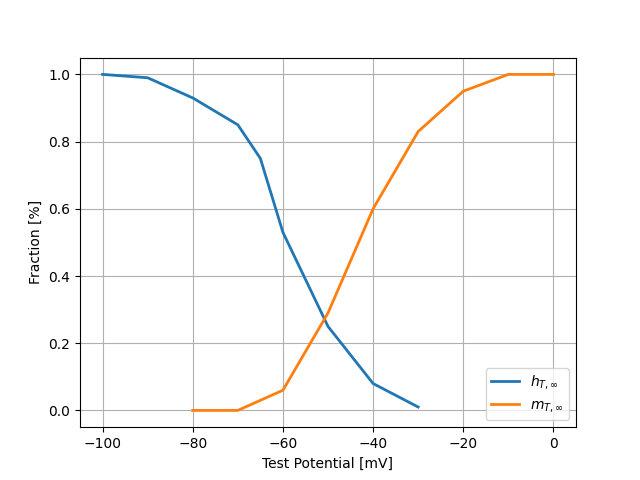
\includegraphics[width=\textwidth]{./img/t_type_calcium_channel/1_activation_and_inactivation_curves.png}
        \caption{}
    \end{subfigure}
    \hfill
    \begin{subfigure}[t]{0.45\textwidth}
        \centering
        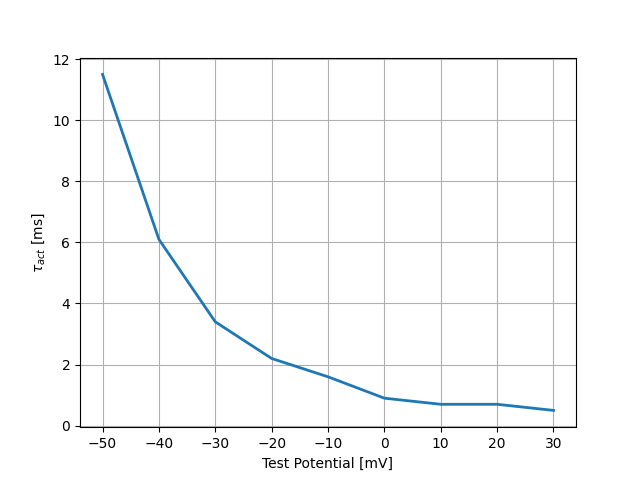
\includegraphics[width=\textwidth]{./img/t_type_calcium_channel/2_1_tau_m_jeong.png}
        \caption{}
    \end{subfigure}
    
    % Second row
    \begin{subfigure}[t]{0.45\textwidth}
        \centering
        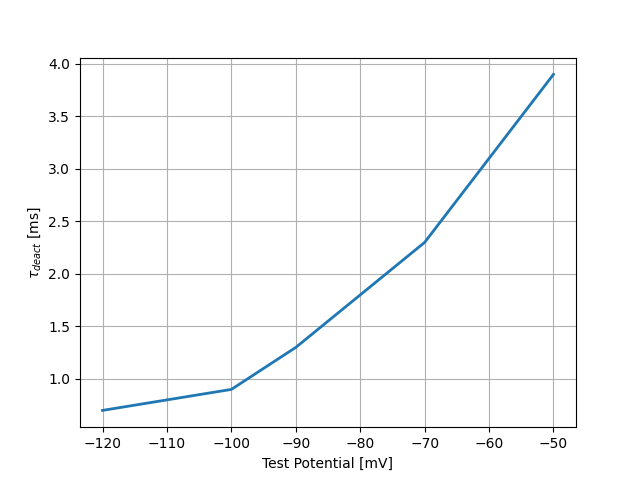
\includegraphics[width=\textwidth]{./img/t_type_calcium_channel/2_1_tau_r_jeong.png}
        \caption{}
    \end{subfigure}
    \hfill
    \begin{subfigure}[t]{0.45\textwidth}
        \centering
        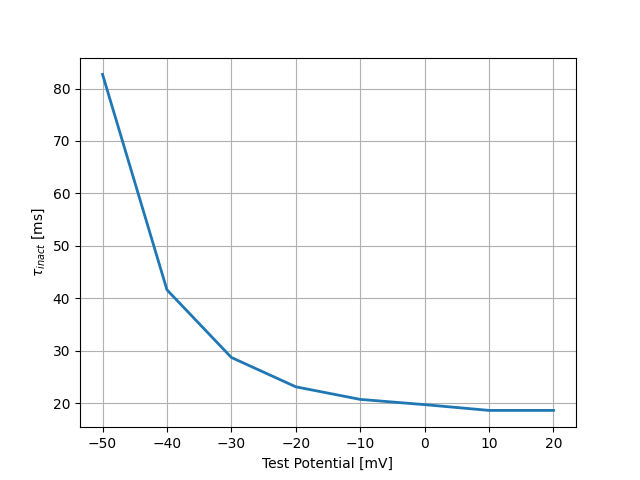
\includegraphics[width=\textwidth]{./img/t_type_calcium_channel/2_1_tau_h_jeong.png}
        \caption{}
    \end{subfigure}
    
    \caption{
        (a) Steady-state activation and inactivation functions of T-type Ca$^{2+}$ channel;
        (b) Activation, (b) deactivation and (c) inactivation as a functions of test potentials.
        Data adapted from \parencite{jeongCaa1TFlyTtype2015}.
    }
    \label{fig:data_from_jeong}
\end{figure}


\begin{note}
    The error due to the subjective visual inspection should not be large. I did not estimated the
    error, but with moving the manually placed dot over the image on the did not have considerable
    effect in the final values (within the moving range where the manually placed dots were not
    obviously not overlapping with the ones from the image).

    The values of the resulted estimates (plotted in the figures above) are provided in
    Section \ref{sec_estimates_of_jeong_2015}.
\end{note}


\subsubsection{Estimating Steady-State Activation/Inactivation Function}

Parameters for steady-state activation variable were estimated by fitting
$m_{T,\infty}^3(V)$ (see Equation \ref{eq_model_r5_t_type_steady_state_activation}) to the data
from electrophysiological recordings presented in \parencite{jeongCaa1TFlyTtype2015} (similar to
the procedure described in \parencite{coulterCalciumCurrentsRat1989}). The steady-state inactivation
was estimated by fitting Equation \ref{eq_model_r5_t_type_steady_state_inactivation} to the
data from the same paper.

\begin{figure}[htbp]
    \centering
    % First row
    \begin{subfigure}[t]{0.45\textwidth}
        \centering
        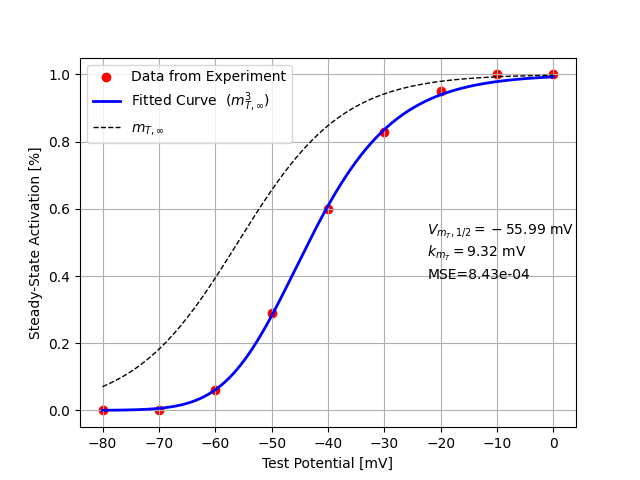
\includegraphics[width=\textwidth]{./img/t_type_calcium_channel/3_fitted_steady_state_activation.png}
    \end{subfigure}
    \hfill
    \begin{subfigure}[t]{0.45\textwidth}
        \centering
        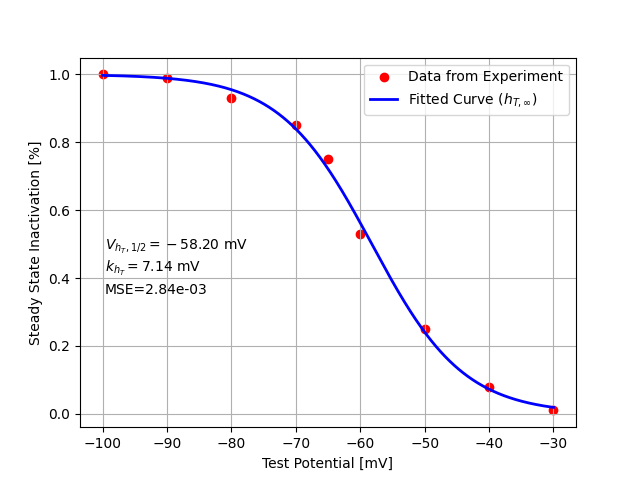
\includegraphics[width=\textwidth]{./img/t_type_calcium_channel/5_fitted_steady_state_inactivation.png}
    \end{subfigure}
    
    \caption{Fitted data to \parencite{jeongCaa1TFlyTtype2015}.}
    \label{fig:data_steady_state_from_jeong}
\end{figure}


\subsubsection{Estimating Activation/Inactivation Time Constants}\label{sec_model_t_type_channel_time_constants}

The data was taken from \parencite{jeongCaa1TFlyTtype2015}. The paper provides
information about the values for activation/inactivation variables, as well as time constants
as a functions of membrane potentials. 

\textbf{Activation time constant}

$a_{T,1}$, $b_{T,1}$, $k_{T,1}$, $a_{T,2}$, $b_{T,2}$, $k_{T,2}$ parameters were fit to the activation
($V \geq -50$ mV) and deactivation ($V < -50$ mV) time constants provided in \parencite{jeongCaa1TFlyTtype2015}
(equations \ref{eq_model_r5_t_type_tau_m_discontinuous}).
The initial guess for the parameters were chosen to be 0, -120, 1 for $a_{T,1}$, $b_{T,1}$, $k_{T,1}$,
and 0, 50, 1 for $a_{T,2}$, $b_{T,2}$, $k_{T,2}$, correspondingly. The results are shown in Figure
\ref{fig:data_fitted_taus_from_jeong_activation}.

\parencite{jeongCaa1TFlyTtype2015} estimated the activation time constant ($V>-50$ mV) by fitting
sum of two exponentials to the recorded current trace. As it is shown in Section \ref{appendix_from_current_to_exp_sum},
the fitted time constant does not need adjustment to account for the correspondingly
time constant of activation. However, the deactivation time constant needs an adjustment.

The authors estimated deactivation time constant by measuring decay of the tail current ($\tau_{\text{tail}}$).
As the model consists of three activation gates, and closing of each ion channel reuires
only one activation gate to close, the deactivation time constant for one gate (out of the three)
will be three times as large as $\tau_{\text{tail}}$ \parencite{huguenardSimulationCurrentsInvolved1992}.
For this reason, $\tau_{m_t}$ for $V<-50$ mV was determined as $3\times\tau_{\text{tail}}$.

As the set of equations \ref{eq_model_r5_t_type_tau_m_discontinuous} have jump discontinuity at
$V=-50$mV, $\sigma_{m_T}$ was introduced to model a smooth transition between the functions
describing the time constant below and above $-50$mV (equation \ref{eq_model_r5_t_type_channel_tau_m_sigma}).
The parameters of the exponentials modeling activation and deactivation time constants were
fixed, and the parameter $c_{\tau_m,T}$ of $\sigma_{m_T}$ was fitted to the combined data of activation
and deactivation time constants from \parencite{jeongCaa1TFlyTtype2015} (Figure \ref{fig:data_fitted_tau_m_from_jeong_smooth_transition}).

\begin{note}
    Original paper for the base model of the R5 neuron \parencite{wangMultipleDynamicalModes1994} did not
    model the activation time constant of T-Type Ca$^{2+}$ channels, as they replaced the
    activation variable by its steady state equation $m_{t,\infty}(V)$.
\end{note}

\begin{note}
    \parencite{destexheVivoVitroComputational1996} fitted activation time constant to double exponentials:
    \begin{equation}\label{eq:fitting_t_type_activation_delay_with_double_exponential}
        \tau_{m_T} = a_{\tau_{m_T}} + \frac{b_{\tau_{m_T}}}{ \exp{[(V - V_{\tau_{m_T}^1,1/2})/k_{\tau_{m_T^1}}]} + \exp{[-(V - V_{\tau_{m_T}^2,1/2})/k_{\tau_{m_T^2}}]}}
    \end{equation}
    However, MSE in case of double exponential fit was larger than with fitting the activation time constant with
    two exponential (see Fig. ), as described above.
\end{note}


\textbf{Inactivation time constant}

\parencite{jeongCaa1TFlyTtype2015} did not provide experimental values for $\tau_{h_T}$ below $-50$mV.
Several authors reported recovery time constant for deinactivation to be much slower than the one of inactivation
\parencite{huguenardNovelTtypeCurrent1992, destexheVivoVitroComputational1996, huguenardSimulationCurrentsInvolved1992}.
Equation \ref{eq_model_r5_t_type_tau_inactivation} is a negative sigmoid, with a left
asymtote at $V\approx216$mV (Figure \ref{fig:data_fitted_taus_from_jeong_inactivation}).

\begin{note}
    Another approach would be to fit the time constant only above $-50$mV and take
    values below $-50$mV from another source (e.g. \parencite{huguenardSimulationCurrentsInvolved1992}).
    However, as 1) the values for Drosophila T-Type channel are not available below $-50$mV,
    2) the fitted time constant has the same order of magnitude below $-50$mV as described
    in the literature for deinactivation time constant, 3) given the previous comment, the
    exact velues will only affect time course of the current and is not very relevant for the
    neuronal model - continuous function was preferred for modeling the inactivation time constant.
\end{note}

\begin{figure}[H]
    \centering
    \begin{subfigure}[t]{0.45\textwidth}
        \centering
        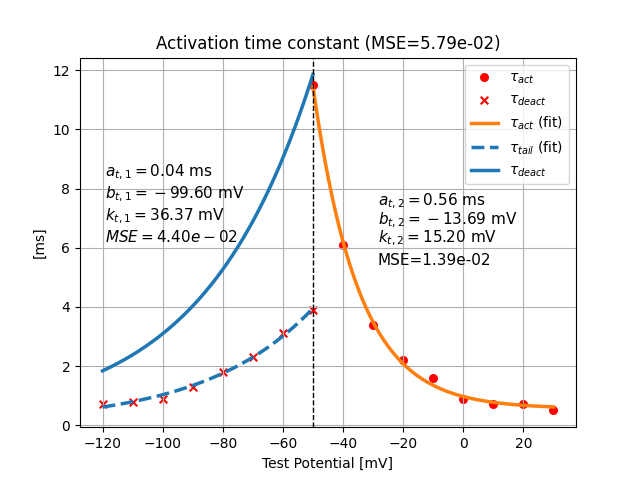
\includegraphics[width=\textwidth]{./img/t_type_calcium_channel/final_tau_activation_fit.png}
        \caption{Fitted activation and deactivation time constants using exponential functions}
        \label{fig:data_fitted_taus_from_jeong_activation}
    \end{subfigure}
    \hfill
    \begin{subfigure}[t]{0.45\textwidth}
        \centering
        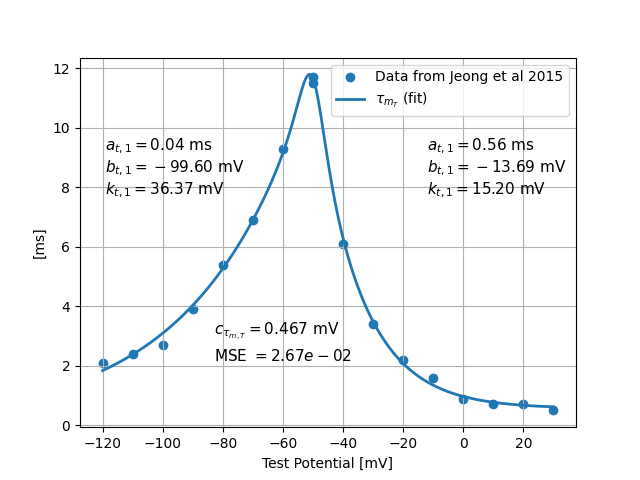
\includegraphics[width=\textwidth]{./img/t_type_calcium_channel/tau_activation_join_exponentials.png}
        \caption{Smooth transition between activation and deactivation time constants}
        \label{fig:data_fitted_tau_m_from_jeong_smooth_transition}
    \end{subfigure}
    
    \caption{Fitted $\tau_{m_T}$ to data from \parencite{jeongCaa1TFlyTtype2015}.}
    \label{fig:data_fitted_taus_from_jeong}
\end{figure}

\begin{figure}[H]
    \centering
    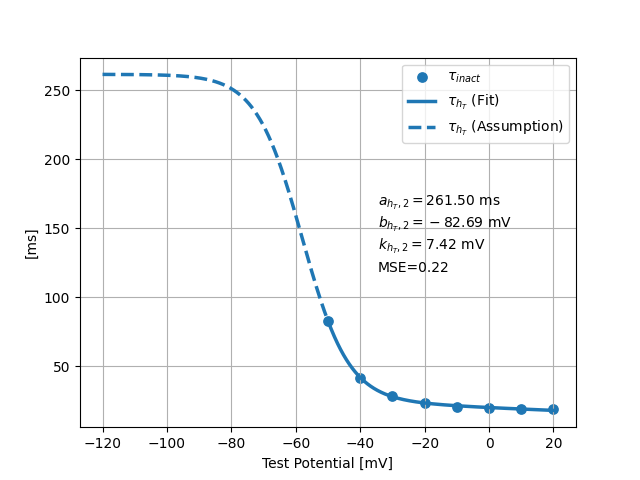
\includegraphics[width=0.45\textwidth]{./img/t_type_calcium_channel/inactivation_tau_fit_2.png}
    \caption{Fitted inactivation time constant}
    \label{fig:data_fitted_taus_from_jeong_inactivation}
\end{figure}

\FloatBarrier


\subsection{Simulations of T-Type \texorpdfstring{Ca$^{2+}$}{Ca+2} Current}\label{subsec_r5_simulations_t_type_current}

Simulations were done using python package '\textit{scipy.integrate.solve\_ivp}' with
zero initial conditions. Different integration methods were compared: RK45, BDF, and LSODA.
Each solver is optimized for different problems (stiff, non-stiff, etc.). Simulations
showed, that for some cases (e.g. simulating only t-type channel) it is best to use
RK45. For the simulatins presented in this section, RK45 method was used.

\subsubsection{Ohmic Current vs Constant-Field Equation}

\color{orange}

\begin{itemize}
    \item How can one fit voltage-current (I-V) relationship?
    \begin{itemize}
        \item Ohmic current: $I(V) = g(V) (V - V_{ion})$, where $g(V) = \hat{g} m_T(V)^3 h_T(V)$, $g$ is conductance,
        $\hat{g}$ maximal conductance, $m_T(V)$ ($h_T(V)$) is variable corresponding to
        activation (inactivation) gate.
        \item Constant field equation (also known as Goldman-Hodgkin-Katz (GHK) voltage flux equation): Equation \ref{eq_constant_field_equation}
        \item The recorded voltage traces and transient I-V relationship to voltage steps is given in Figure \ref{fig:i_v_relationship_jeong}.
        \item Voltage step protocol: The membrane potential was held at holding potential $-90$ mV,
        followed by $150$ms step pulses that varied from $-80$-$40$mV with $10$mV increments
        (see e.g. Figure \ref{fig_t_type_ohmic_voltage_traces}, second plot from top). The response
        of the neuron to the voltage steps was recorded (see e.g. Figure \ref{fig_t_type_ohmic_voltage_traces}, second figure from top).
        \item Observed I-V relationship was replicated for GHK model, but not for Ohmic current
        (Figure \ref{fig_t_type_voltage_step_ohmic_vs_constant_field}).
        % \item The sharp transient at the end of the pulse in recordings (Fig. \ref{fig:i_v_relationship_jeong})
        % is most likely due to passive membrane properties. The membrane time constant of R5 neuons is not known.
        % Arbitrarily incorporating $\tau=10$ms time constant reproduced the sharp transient (not shown here).
        % However 1) as Drosophila T-Type channels were expressed in frogs (Oocites), fitting membrane time constant
        % will not be helpful in modeling Drosophila R5 neurons; 2) The passive membrane time constant
    \end{itemize}
\end{itemize}

\color{black}

\textcolor{red}{Add text, add captions in figure \ref{fig_t_type_voltage_step_ohmic_vs_constant_field}}.

\begin{figure}[H]
    \centering
    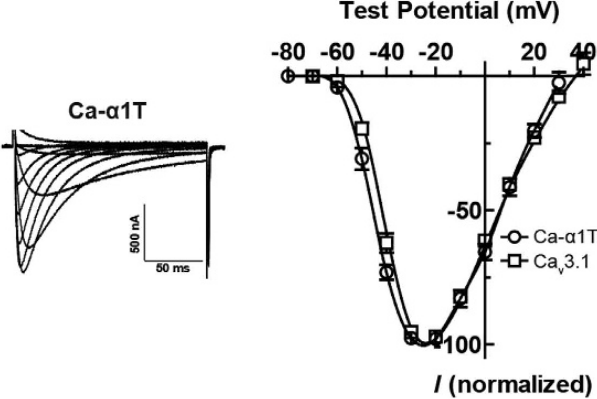
\includegraphics[width=0.45\textwidth]{./img/t_type_calcium_channel/iv_relationship_jeong_2015.png}
    \caption{I-V relationship of T-Type Ca$^{2+}$ current in Drosophila. Adapted from \parencite{jeongCaa1TFlyTtype2015}.}
    \label{fig:i_v_relationship_jeong}
\end{figure}

\begin{figure}[H]
    \centering
    % First row
    \begin{subfigure}[t]{0.45\textwidth}
        \centering
        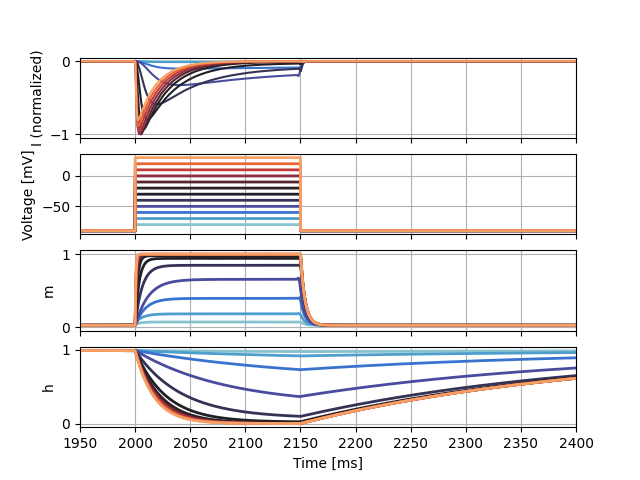
\includegraphics[width=\textwidth]{./img/t_type_calcium_channel/simulations/No Scale/Ohm's LawVoltage Step Up-Down6_voltage_traces.png}
        \caption{}
        \label{fig_t_type_ohmic_voltage_traces}
    \end{subfigure}
    \hfill
    \begin{subfigure}[t]{0.45\textwidth}
        \centering
        \includegraphics[width=\textwidth]{./img/t_type_calcium_channel/simulations/No Scale/Constant Field EquationVoltage Step Up-Down6_voltage_traces.png}
        \caption{}
        \label{fig_t_type_constant_field_voltage_traces}
    \end{subfigure}

    % Second row
    \begin{subfigure}[t]{0.45\textwidth}
        \centering
        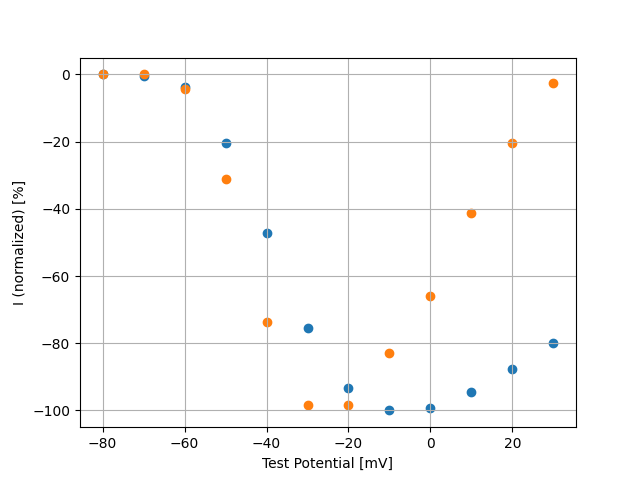
\includegraphics[width=\textwidth]{./img/t_type_calcium_channel/simulations/No Scale/Ohm's LawVoltage Step5_IV_Relationship_comparison_Jeong_2015.png}
        \caption{}
        \label{fig_t_type_ohmic_iv_relationship}
    \end{subfigure}
    \hfill
    \begin{subfigure}[t]{0.45\textwidth}
        \centering
        \includegraphics[width=\textwidth]{./img/t_type_calcium_channel/simulations/No Scale/Constant Field EquationVoltage Step5_IV_Relationship_comparison_Jeong_2015.png}
        \caption{}
        \label{fig_t_type_constant_field_iv_relationship}
    \end{subfigure}
    
    \caption{Ohm's low vs constant-field equation for T-Type Ca$^{2+}$ current.}
    \label{fig_t_type_voltage_step_ohmic_vs_constant_field}
\end{figure}


\subsubsection{Scaling/Shifting Gating Variables}

\color{red}

\begin{itemize}
    \item $[Ca]_{outside}$, as well as solutions used during voltage-clamp experiments
    (calcium vs barium, as well as corresponding concentations) affects gating constants,
    including for mammalian homologes of Drosophila T-Type Ca channels.
    \item To my knowledge, how exactly the time constants are affected for Drosophila T-Type Ca channels
    has not been reported.
    \item For now: shifted steady state activation and scaled tau activation (python function curve\_fit
    with initial guesses p0=[4, 0.5] for shift and scale correspondingly)
    \item m(v) to m(v-4.95)
    \item tau to tau*0.45
\end{itemize}

\color{black}

\begin{figure}[H]
    \centering
    % First row
    \begin{subfigure}[t]{0.45\textwidth}
        \centering
        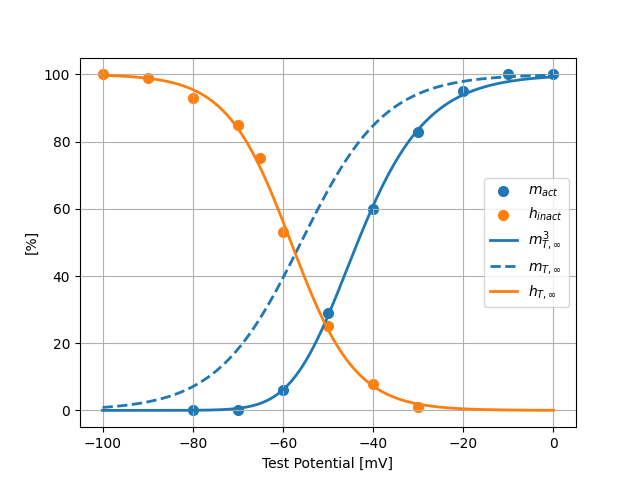
\includegraphics[width=\textwidth]{./img/t_type_calcium_channel/simulations/Scaling/Constant Field Equation1_steady_state_activation_inactivation.png}
        \caption{}
        \label{fig_r5_t_type_steady_state_activation_shifted}
    \end{subfigure}
    \hfill
    \begin{subfigure}[t]{0.45\textwidth}
        \centering
        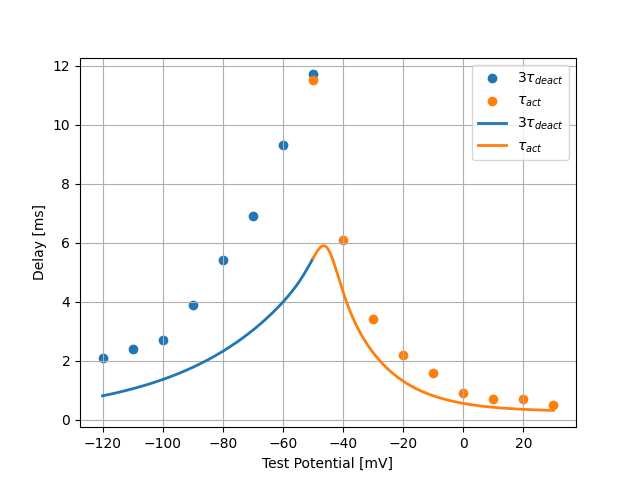
\includegraphics[width=\textwidth]{./img/t_type_calcium_channel/simulations/Scaling/Constant Field Equation2_tau_m.png}
        \caption{}
        \label{fig_r5_t_type_tau_activation_scaled}
    \end{subfigure}
    
    \caption{\textcolor{red}{Shifting and scaling time constants of activation gate}}
    \label{fig_r5_t_type_shifting_scaling}
\end{figure}

\begin{figure}[H]
    \centering
    % First row
    \begin{subfigure}[t]{0.45\textwidth}
        \centering
        \includegraphics[width=\textwidth]{./img/t_type_calcium_channel/simulations/Scaling/Constant Field EquationVoltage Step Up-Down6_voltage_traces.png}
        \caption{}
        \label{fig_t_type_constant_field_voltage_traces_scaled}
    \end{subfigure}
    \hfill
    \begin{subfigure}[t]{0.45\textwidth}
        \centering
        \includegraphics[width=\textwidth]{./img/t_type_calcium_channel/simulations/Scaling/Constant Field EquationVoltage Step5_IV_Relationship_comparison_Jeong_2015.png}
        \caption{}
        \label{fig_t_type_constant_field_iv_relationship_scaled}
    \end{subfigure}
    
    \caption{\textcolor{red}{Reconstructed I-V relationship after scaling and shifting activation gate time constant}}
    \label{fig_t_type_voltage_step_ohmic_vs_constant_field_scaled}
\end{figure}


\newpage
\subsection{Appendix}

\subsubsection{Estimates of Data in Jeong et al 2015}\label{sec_estimates_of_jeong_2015}

\begin{figure}[H]
    \centering
    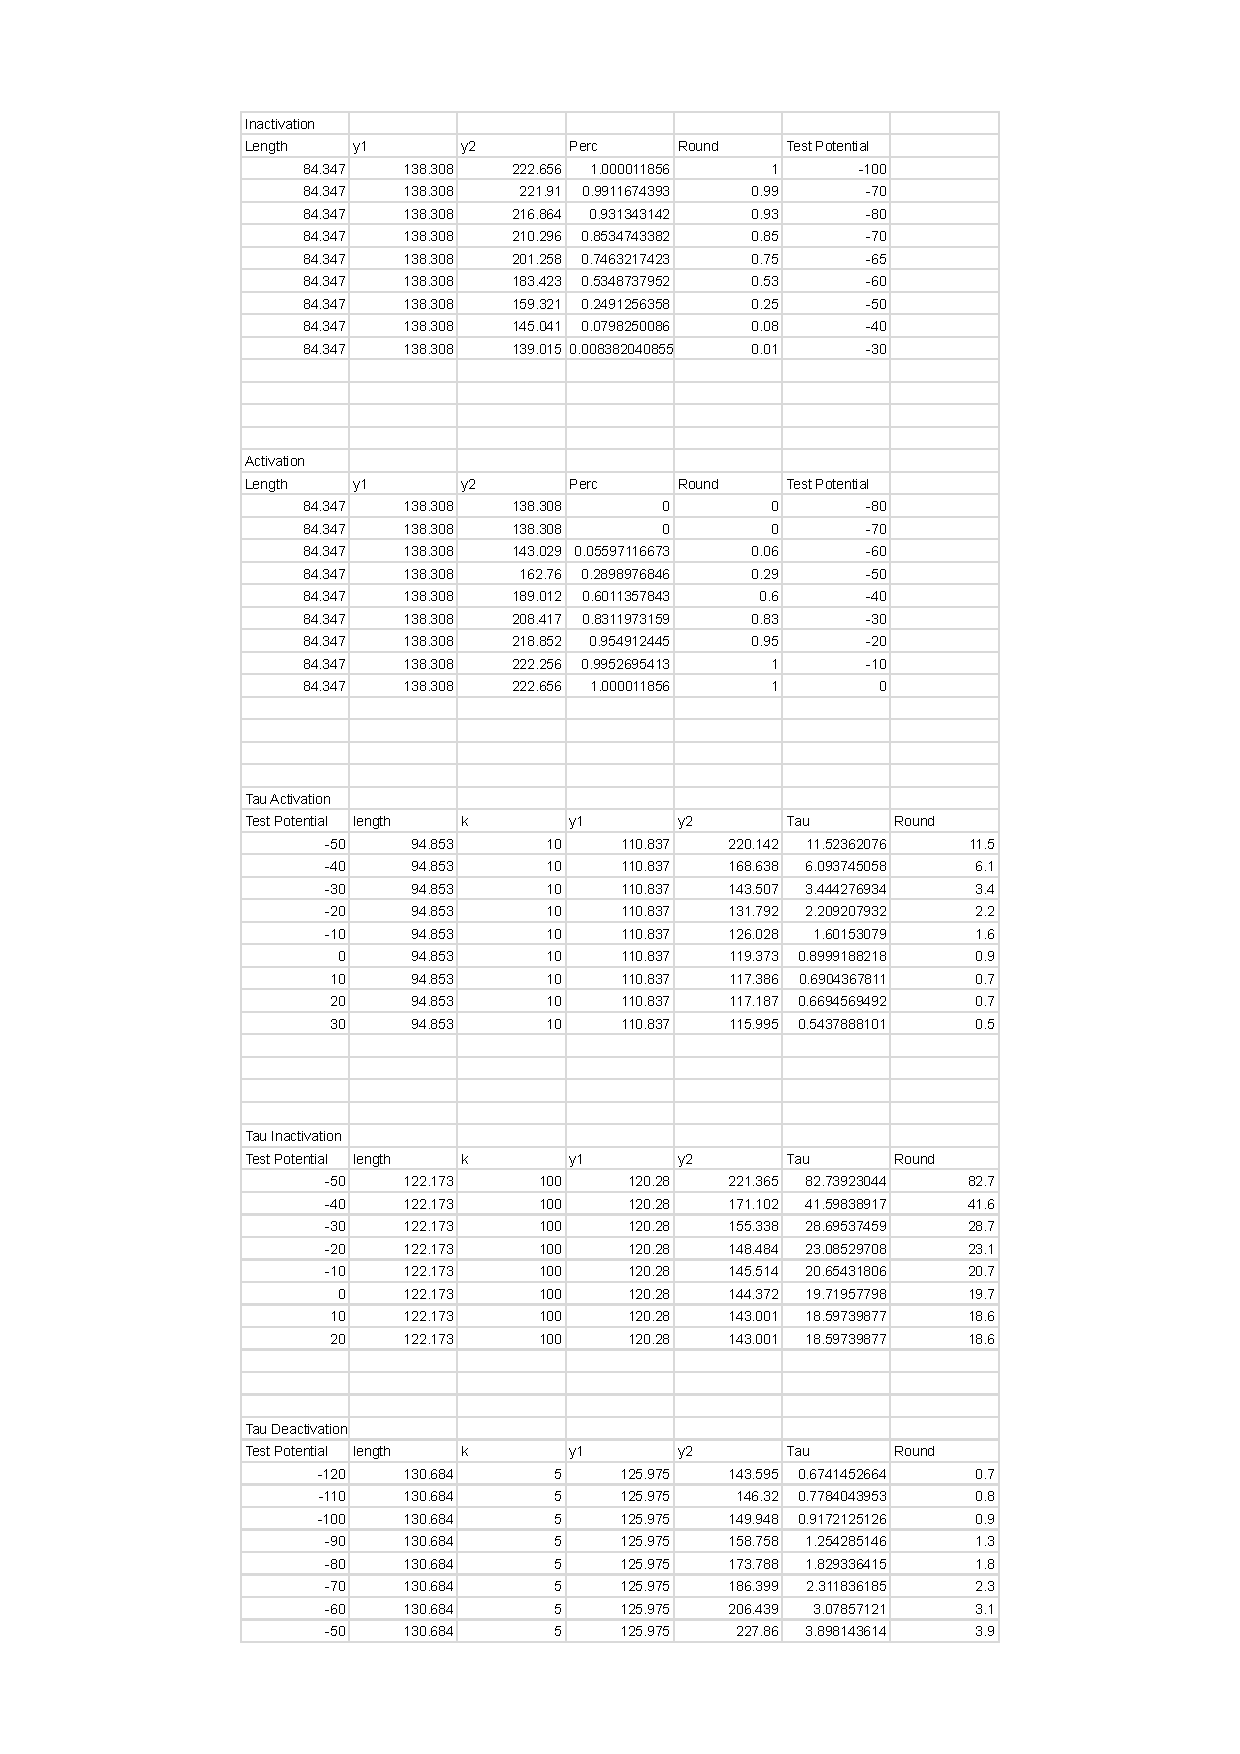
\includegraphics[height=0.9\textheight]{Handwritten Notes/R5 Model/T Type (Jeong) - Activation_Inactivation.pdf}
\end{figure}

\subsubsection{From Current Trace to Sum of Exponentials}\label{appendix_from_current_to_exp_sum}
\begin{figure}[H]
    \centering
    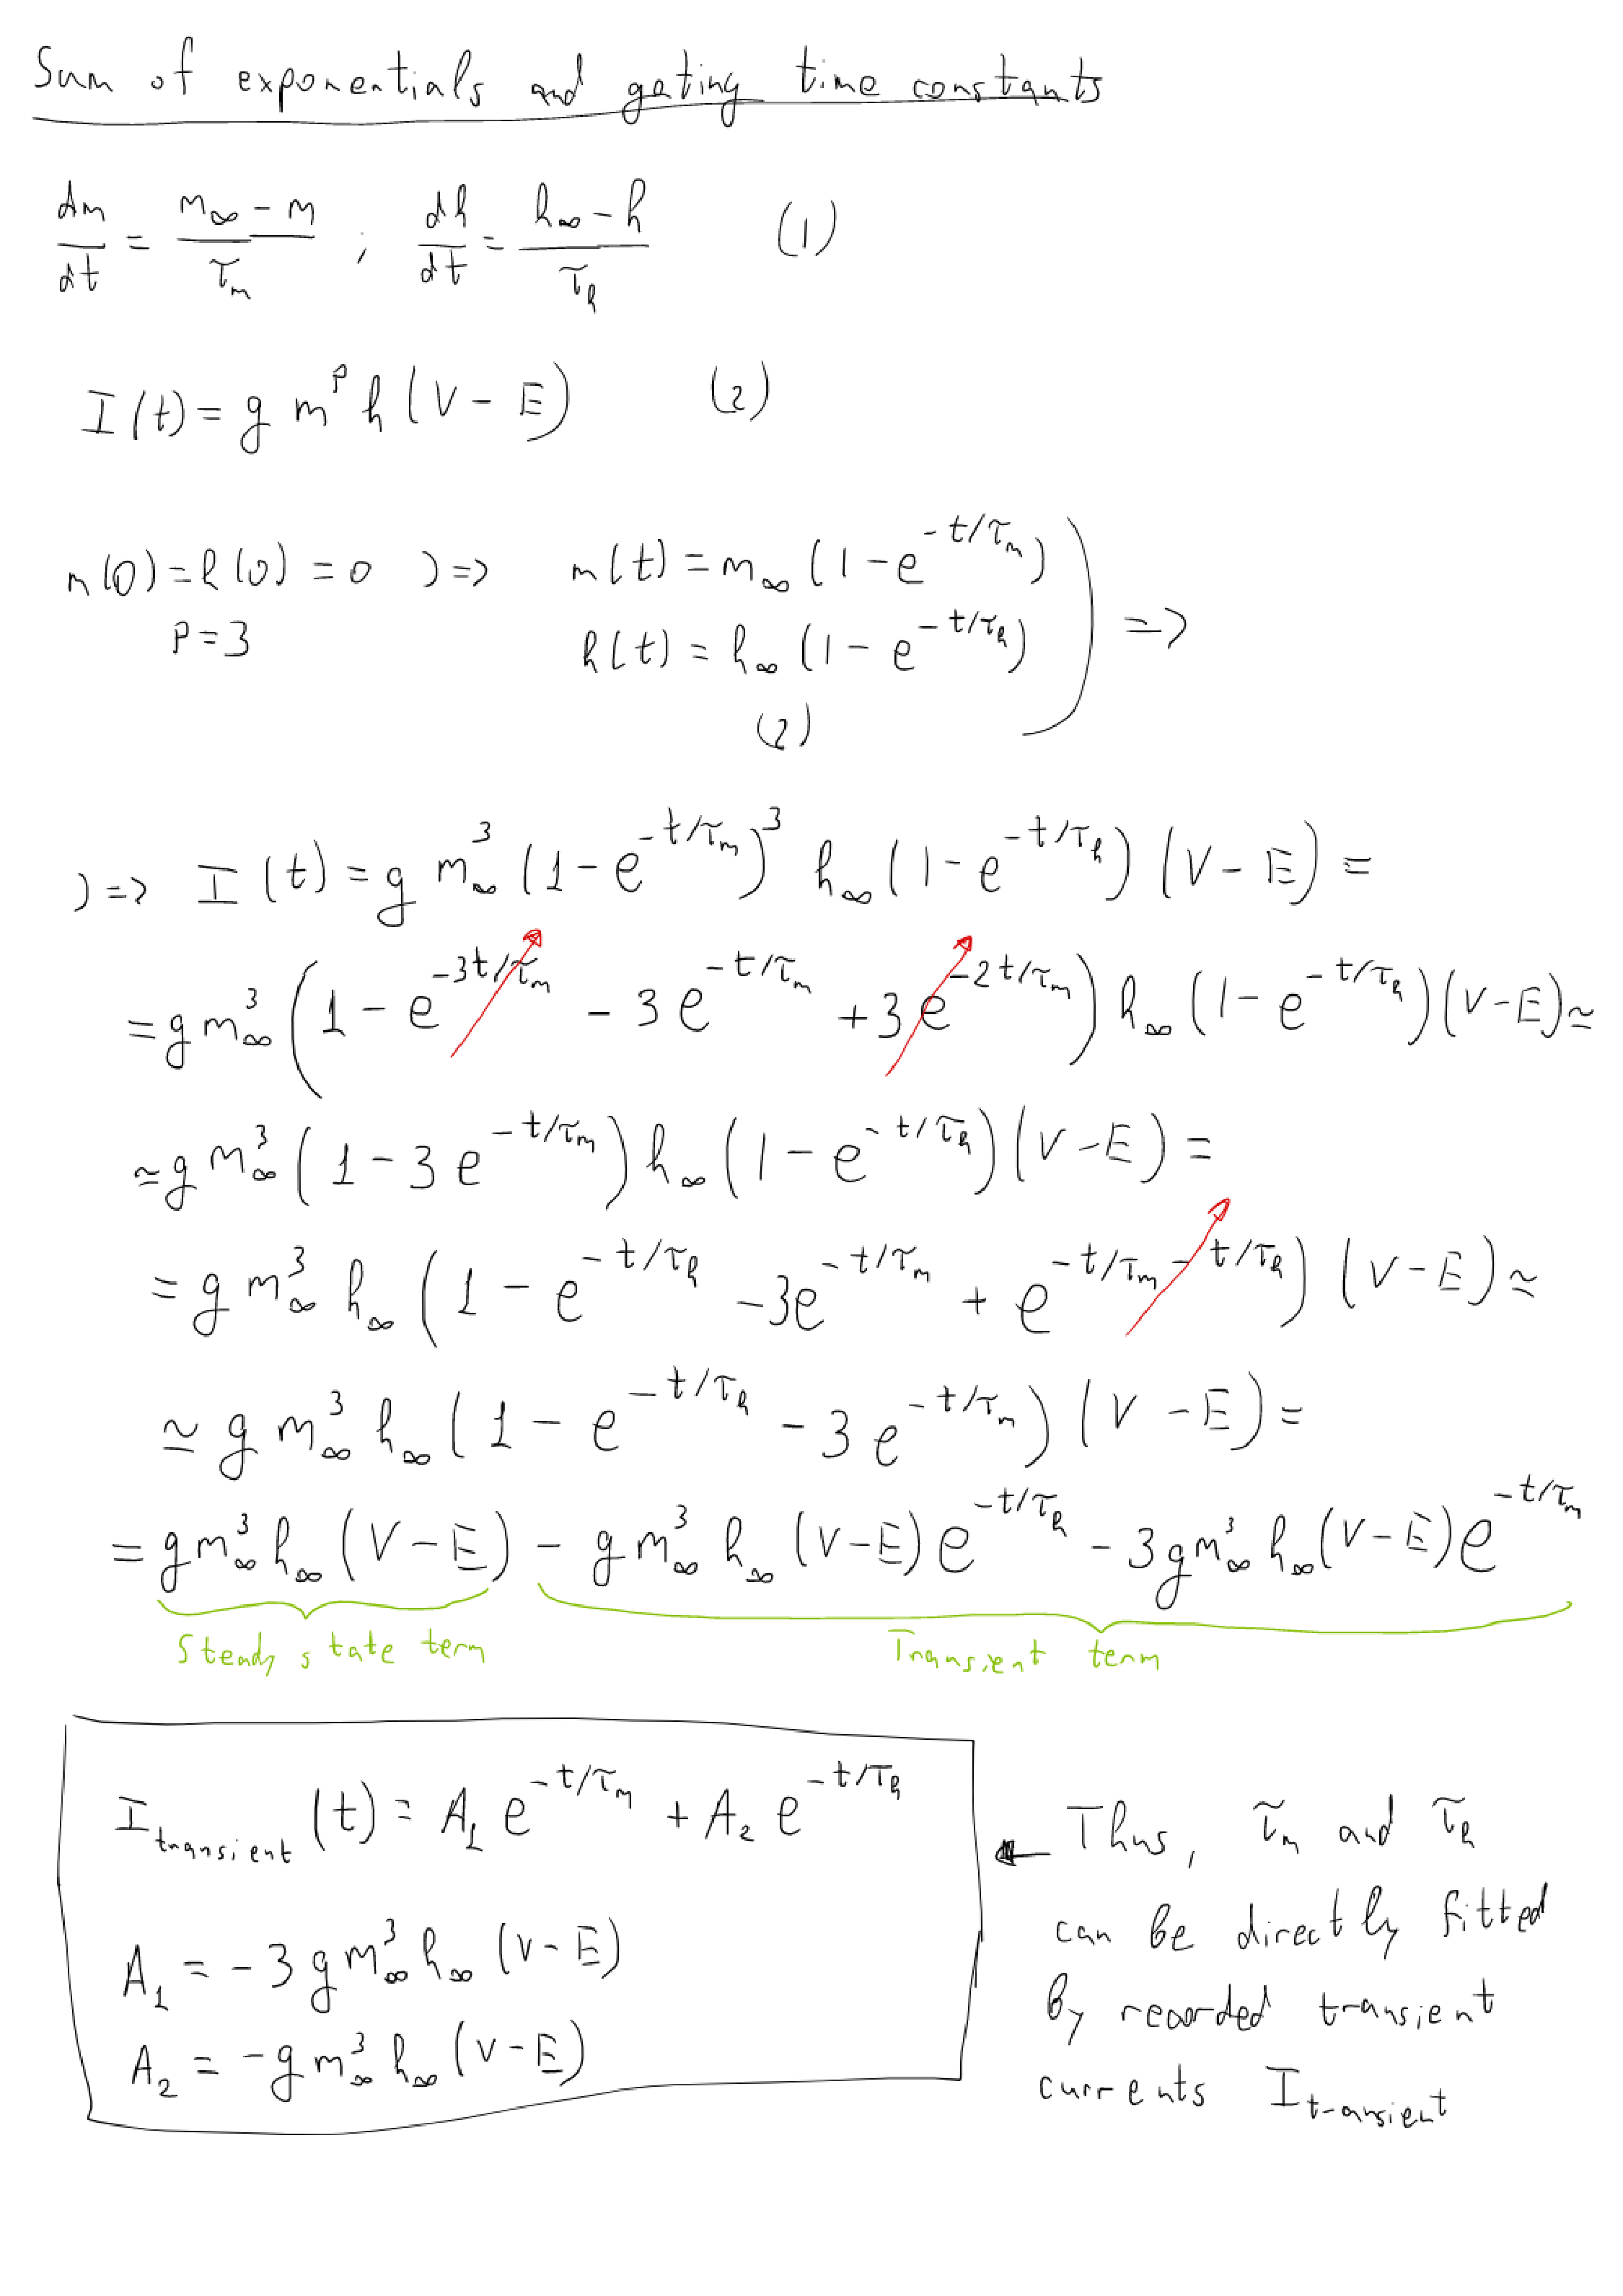
\includegraphics[height=0.9\textheight]{Handwritten Notes/R5 Model/Z1 - Double exponential fit to transient current.pdf}
\end{figure}

\newpage
\subsubsection{Derivation of equations in Wang 1991}\label{sec_derivation_wang_1991}
\begin{figure}[H]
    \centering
    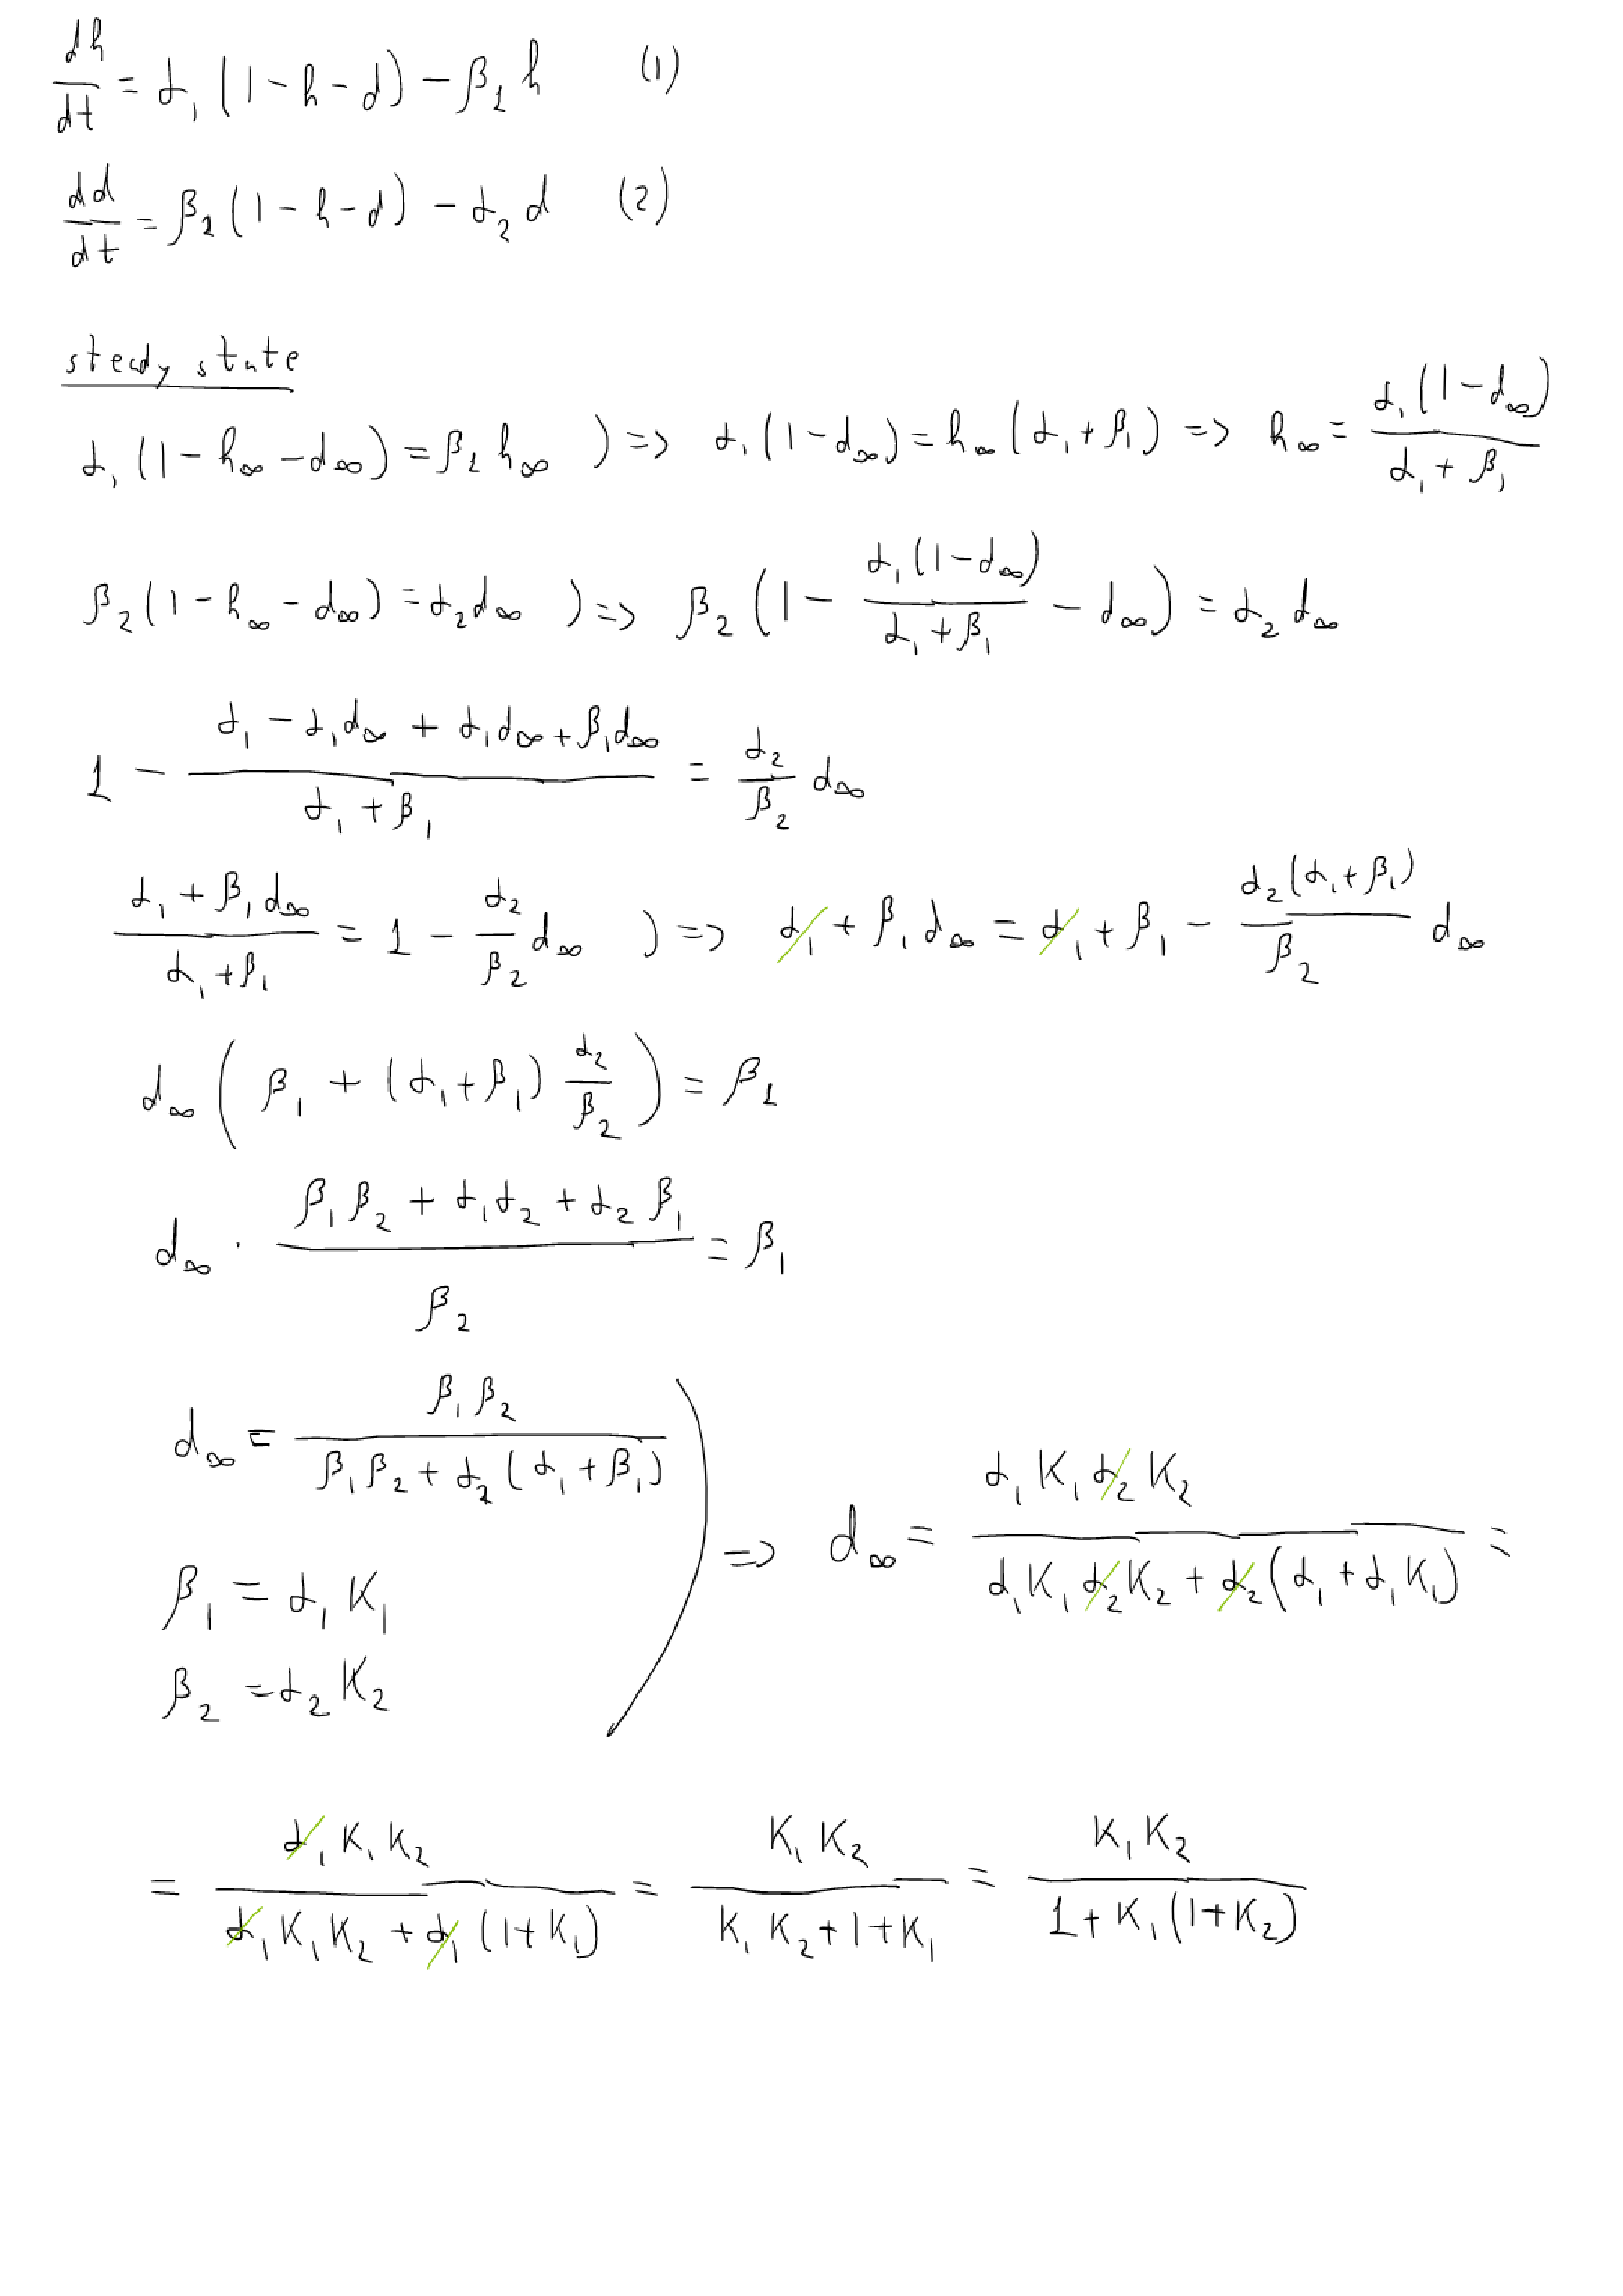
\includegraphics[height=0.9\textheight, page=1]{Handwritten Notes/R5 Model/Z2 - Notes Wang 1991 T-Type.pdf}
\end{figure}


% Insert the PDF and apply custom page numbering for the footer
\includepdf[pages=2-,height=\textheight,pagecommand={
  \thispagestyle{mypdfstyle}  % Apply custom footer with page number
}]{Handwritten Notes/R5 Model/Z2 - Notes Wang 1991 T-Type.pdf}


\newpage
\subsubsection{Overcoming Singularities in Constant-Field Equation}
\begin{figure}[H]
    \centering
    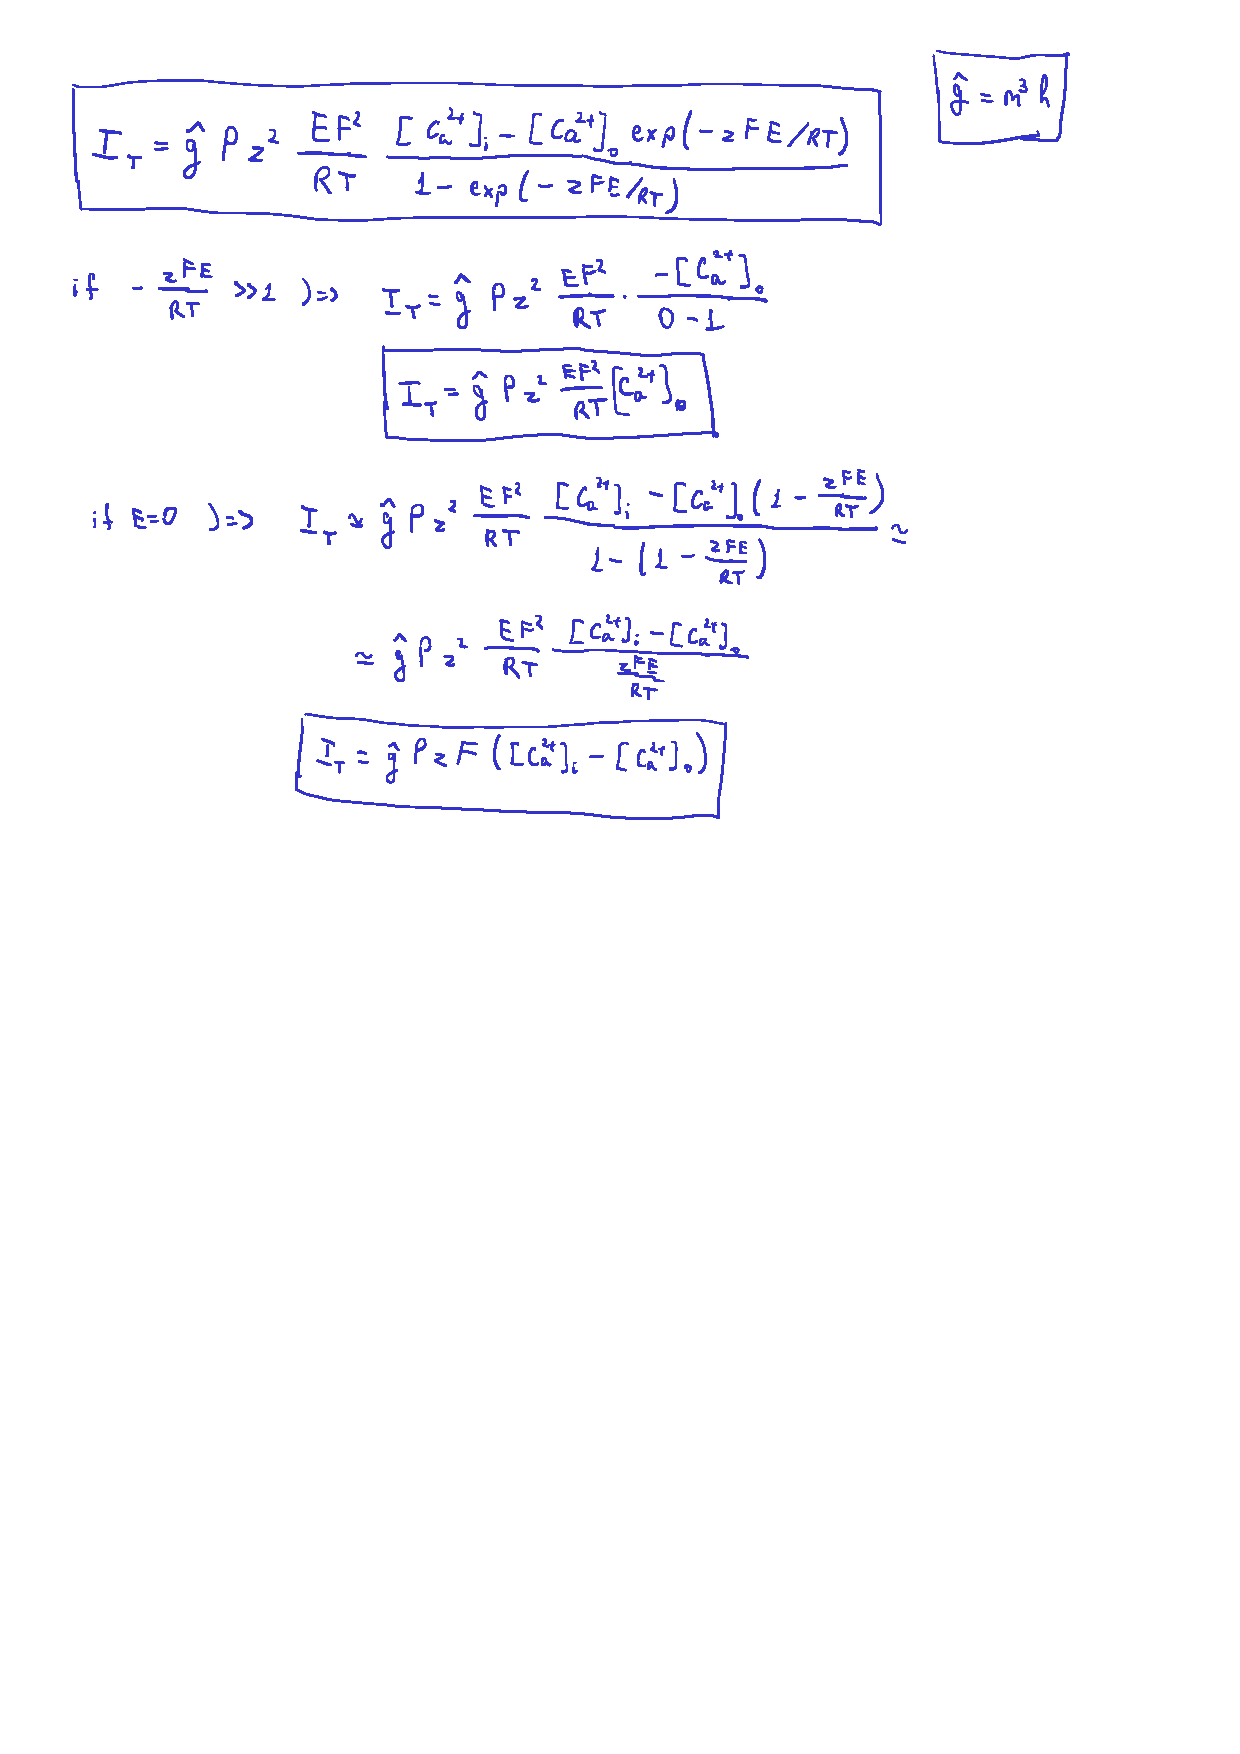
\includegraphics[height=0.9\textheight, page=1]{Handwritten Notes/R5 Model/Singularities in Constant-Field Equation.pdf}
\end{figure}

\newpage
\subsubsection{Additional Figures}
\begin{figure}[H]
    \centering
    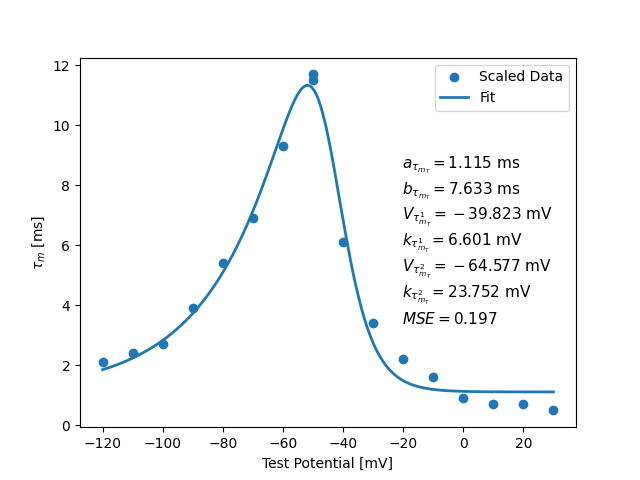
\includegraphics[width=0.5\textwidth, page=1]{./img/t_type_calcium_channel/activation_fit_by_double_exponentials.png}
    \caption{
        Fitting time constant of activation function for T-Type Ca$^{2+}$ channel by double exponential function
        (Eq. \ref{eq:fitting_t_type_activation_delay_with_double_exponential}). The fitting was done using the Python
        library \textit{scipy.optimize.curve\_fit} with the following initial guesses for the parameters:
        $a_{\tau_{m_T}}=2$, $b_{\tau_{m_T}}=1$, $V_{\tau_{m_T}^1}=-100$, $k_{\tau_{m_T}^1}=10$,
        $V_{\tau_{m_T}^2}=-40$, $k_{\tau_{m_T}^2}=10$.
    }
\end{figure}

\newpage
\printbibliography

\end{document}